\documentclass[8pt, handout]{beamer} 


%% Math packages
%%
\usepackage{amsmath,amsthm,amssymb}
% Removes the "Too many math alphabets used in version normal" error.
\newcommand\hmmax{0}
\newcommand\bmmax{0}
\usepackage[new]{old-arrows}
\usepackage{cancel}
\usepackage{mathdots}
\usepackage{venndiagram}
\usepackage{mathrsfs}          % Math script font

% Graphics
%%
\graphicspath{{./}{figs/}}
\usepackage{graphicx}
\usepackage{tikz}
\usetikzlibrary{arrows}
\usetikzlibrary{decorations.markings}
\usetikzlibrary{decorations.pathreplacing}
\usetikzlibrary{patterns}
\usetikzlibrary{shapes.geometric}
\usetikzlibrary{positioning}
\usetikzlibrary{matrix}
\usepackage{tikz-3dplot}
\usepackage{tkz-graph}
\usepackage{tikz-cd}

%% Colors 
%%
\usepackage{xcolor}
\usepackage{color}
\usepackage{visualalgebra}  %% Put this *after* the TikZ packages
\usepackage{visualalgebraslides}  %% Put this *after* "visualalgebra"

%% Page layout packages
%%
\usepackage{url}
\usepackage{multicol}
\usepackage{multirow}
\usepackage[numbers,square,sort&compress]{natbib}

%% Font and formatting packages
%%
\usepackage[english]{babel}    % Removing this causes compiler error
\usepackage{alltt}             % Like verbatim, but excludes \ and { }
\usepackage{enumerate}         % [shortlabels] option??
\usepackage{comment}
\usepackage{soul}              % strikeout text
\usepackage{bm}                % Bold math
\usepackage[T1]{fontenc}
\usepackage{relsize}

%% Fixes the \mathbf{} not working for fonts under 10pt
\usepackage{cmbright}
\fontencoding{OT1}\fontfamily{cmbr}\selectfont %to load ot1cmbr.fd
\DeclareFontShape{OT1}{cmbr}{bx}{n}{% change bx definition
<->cmbrbx10%
}{}
\normalfont

\makeatletter
\renewcommand*\env@matrix[1][\arraystretch]{%
  \edef\arraystretch{#1}%
  \hskip -\arraycolsep
  \let\@ifnextchar\new@ifnextchar
  \array{*\c@MaxMatrixCols c}}
\makeatother


%%=======================================================================

%% Beamer packages
%%
\mode<presentation>
{
  \usetheme{boadilla} 
  \useinnertheme{rectangles}
  \usecolortheme{dolphin}
}

\setbeamersize{text margin left=6mm}
\setbeamersize{text margin right=6mm}
\setbeamersize{sidebar width right=0mm}
\setbeamersize{sidebar width left=0mm}
\setbeamertemplate{navigation symbols}{}

\def\newblock{\hskip .11em plus .33em minus .07em}

% Other options: ball, circle, square 
\setbeamertemplate{enumerate items}[default]
%\setbeamercolor{enumerate subitem}{fg=red!80!black}
\def\opacity{0.5}
%\setbeamercovered{transparent}
\setbeamercovered{invisible}

\newcommand{\Pause}{\pause}      %% Comment this out => lots more page breaks


\AtBeginSection[]{
  \begin{frame}
  \vfill
  \centering
  \begin{beamercolorbox}[sep=8pt,center,shadow=true,rounded=true]{title}
    \usebeamerfont{title}\insertsectionhead\par%
  \end{beamercolorbox}
  \vfill
  \end{frame}
}

%%====================================================================

\title[Applications of group actions!]{Applications of group actions!}

\author[\href{mailto:sbagley@westminsteru.edu}{S. Bagley}]
       {\href{mailto:sbagley@westminsteru.edu}{Spencer Bagley}}

\institute[Westminster] { 
  \normalsize With many thanks to Matthew Macauley, \\
  \url{http://www.math.clemson.edu/~macaule/}}

\date[14 Apr 2025]{14 Apr 2025}

\begin{document}

\frame{\titlepage}

%%====================================================================

\begin{frame}{Overview} %\Pause

  Intuitively, a \Alert{group action} occurs when a group $G$
  ``naturally permutes'' a set $S$ \emph{of states}.

  \medskip

  \begin{block}{Formal definition}
    A group $G$ \Alert{acts on} a set $S$ if there is a homomorphism
    $\phi\colon G\to\Perm(S)$. 

    We'll use \Alert{right group actions},
    
    and we'll write \Alert{$s.\phi(g)$} to denote ``where pushing the $g$-button sends state $s$.''
  \end{block} 

  \begin{block}{Definition}
    A set $S$ with a (right) action by $G$ is called a (right)
    \Alert{$G$-set}.
  \end{block} 
  
  \begin{alertblock}{Big ideas}
   \begin{itemize}
    \item An action $\phi\colon G\to\Perm(S)$ endows $S$ with an
      \textbf{algebraic structure}. 
    \item \emph{\Alert{Action graphs are to $G$-sets}, like how
      \Balert{Cayley graphs are to groups}.}
    \end{itemize}
  \end{alertblock}

  \begin{exampleblock}{Notation}
    Throughout, we'll denote identity elements by $1\in G$ and $e\in\Perm(S)$.
  \end{exampleblock}
  
\end{frame}

%%====================================================================

\begin{frame}{Five features of every group action} %\Pause

  Every group action has \textbf{five fundamental features} that we
  will always try to understand. \medskip

  \begin{tabular}{|l|l|l|}
    \hline
    & \Alert{local} (about an $s$ or a $g$)
    & \Palert{global} (about the whole action $\phi$)
    \\\hline
    subsets of $S$   & \begin{tabular}[c]{@{}l@{}}$\Alert{\orb(s)}$ \\ $\Galert{\fix(g)}$ \end{tabular} & $\Galert{\Fix(\phi)} = \displaystyle\bigcap_{g\in G} \Galert{\fix(g)}$ \\ \hline
    subgroups of $G$ & $\Balert{\stab(s)}$ & $\Balert{\Ker(\phi)} = \displaystyle\bigcap_{s\in S} \Balert{\stab(s)} $       \\ \hline
  \end{tabular}

  \medskip

  ``Duality:'' \Balert{columns} vs. \Galert{rows} in the fixed-point table:
  \begin{itemize}
    \item the \Balert{stablizers} can be read off the \Balert{columns}:
    \emph{group elements that \underline{fix} $s\in S$} \smallskip
    \item the \Balert{kernel} is the rows with a check in \Balert{every column} \smallskip
    \item the \Galert{fixators} can be read off the \Galert{rows}:
    \emph{set elements \underline{fixed by} $g\in G$} \smallskip
    \item the \Galert{fixed points} are the columns with a check in \Galert{every row}
  \end{itemize}

  \medskip

\end{frame}

%%====================================================================

\begin{frame}{Fixed-point tables}
  
    Here is the fixed-point table for $G = D_4$ acting on $S$ the list of 7 ``binary squares.''
    
    %% Fixed point table of our binary square example
    \[
    \renewcommand\arraystretch{1.8}
    \begin{tabular}{c|cccccccccccccc}
      && \begin{tikzpicture}[scale=.5]
           \tikzstyle{every node}=[font=\scriptsize]
           \path[fill=actOrange] (0,.5) rectangle ++(.5,.5); 
           \path[fill=actOrange] (.5,.5) rectangle ++(.5,.5);
           \path[fill=actOrange] (0,0) rectangle ++(.5,.5);
           \path[fill=actOrange] (.5,0) rectangle ++(.5,.5);
           \draw (.25,.75) node{$0$};\draw(.75,.75)node{$0$};
           \draw (.25,.25) node{$0$};\draw(.75,.25)node{$0$};
           \draw (0,0) rectangle (1,1); 
         \end{tikzpicture}
      && 
      \begin{tikzpicture}[scale=.5]
        \tikzstyle{every node}=[font=\scriptsize]
        \path[fill=actOrange] (0,.5) rectangle ++(.5,.5); 
        \path[fill=actPurple] (.5,.5) rectangle ++(.5,.5);
        \path[fill=actPurple] (0,0) rectangle ++(.5,.5);
        \path[fill=actOrange] (.5,0) rectangle ++(.5,.5);
        \draw (0,0) rectangle (1,1);
        \draw(.25,.75) node{$0$};\draw(.75,.75)node{$1$};
        \draw(.25,.25) node{$1$};\draw (.75,.25)node{$0$};
      \end{tikzpicture}
      &&
      \begin{tikzpicture}[scale=.5]
        \tikzstyle{every node}=[font=\scriptsize]
        \path[fill=actPurple] (3.5,.5) rectangle ++(.5,.5); 
        \path[fill=actOrange] (4,.5) rectangle ++(.5,.5);
        \path[fill=actOrange] (3.5,0) rectangle ++(.5,.5);
        \path[fill=actPurple] (4,0) rectangle ++(.5,.5);
        \draw (3.5,0) rectangle (4.5,1);
        \draw(3.75,.75) node{$1$};\draw(4.25,.75)node{$0$};
        \draw(3.75,.25) node{$0$};\draw (4.25,.25)node{$1$};
      \end{tikzpicture}
      &&
      \begin{tikzpicture}[scale=.5]
        \tikzstyle{every node}=[font=\scriptsize]
        \path[fill=actOrange] (0,.5) rectangle ++(.5,.5); 
        \path[fill=actOrange] (.5,.5) rectangle ++(.5,.5);
        \path[fill=actPurple] (0,0) rectangle ++(.5,.5);
        \path[fill=actPurple] (.5,0) rectangle ++(.5,.5);
        \draw (0,0) rectangle (1,1);
        \draw (.25,.75) node{$0$}; \draw (.75,.75) node{$0$};
        \draw (.25,.25) node{$1$}; \draw (.75,.25) node{$1$};
      \end{tikzpicture}
      &&
      \begin{tikzpicture}[scale=.5]
        \tikzstyle{every node}=[font=\scriptsize]
        \path[fill=actOrange] (0,.5) rectangle ++(.5,.5); 
        \path[fill=actPurple] (.5,.5) rectangle ++(.5,.5);
        \path[fill=actOrange] (0,0) rectangle ++(.5,.5);
        \path[fill=actPurple] (.5,0) rectangle ++(.5,.5);
        \draw (0,0) rectangle (1,1);
        \draw (.25,.75) node{$0$}; \draw (.75,.75) node{$1$};
        \draw (.25,.25) node{$0$}; \draw (.75,.25) node{$1$};
      \end{tikzpicture}
      &&
      \begin{tikzpicture}[scale=.5]
        \tikzstyle{every node}=[font=\scriptsize]
        \path[fill=actPurple] (0,.5) rectangle ++(.5,.5); 
        \path[fill=actPurple] (.5,.5) rectangle ++(.5,.5);
        \path[fill=actOrange] (0,0) rectangle ++(.5,.5);
        \path[fill=actOrange] (.5,0) rectangle ++(.5,.5);
        \draw (0,0) rectangle (1,1);
        \draw (.25,.75) node{$1$}; \draw (.75,.75) node{$1$};
        \draw (.25,.25) node{$0$}; \draw (.75,.25) node{$0$};
      \end{tikzpicture}
      &&
      \begin{tikzpicture}[scale=.5]
        \tikzstyle{every node}=[font=\scriptsize]
        \path[fill=actPurple] (0,.5) rectangle ++(.5,.5); 
        \path[fill=actOrange] (.5,.5) rectangle ++(.5,.5);
        \path[fill=actPurple] (0,0) rectangle ++(.5,.5);
        \path[fill=actOrange] (.5,0) rectangle ++(.5,.5);
        \draw (0,0) rectangle (1,1);
        \draw (.25,.75) node{$1$}; \draw (.75,.75) node{$0$};
        \draw (.25,.25) node{$1$}; \draw (.75,.25) node{$0$};
      \end{tikzpicture}
      \\ 
      \hline $1$ && \checkmark && \checkmark && \checkmark && \checkmark && \checkmark && \checkmark && \checkmark  \\
      $r$ && \checkmark && && && && && && \\
      $r^2$ && \checkmark && \checkmark && \checkmark && && && && \\
      $r^3$ && \checkmark && && && && && && \\
      $f$ && \checkmark && && && \checkmark && && \checkmark && \\
      $rf$ && \checkmark && \checkmark && \checkmark && && && && \\
      $r^2f$ && \checkmark && && && && \checkmark && && \checkmark \\
      $r^3f$ && \checkmark && \checkmark && \checkmark && && && && 
      %\hline \\
    \end{tabular}
    \]

    \pause

    $\Balert{\Ker(\phi)} = \{1\}$ and $\Galert{\Fix(\phi)} = \{$ the 0 0 0 0 one$\}$.
\end{frame}

%%====================================================================

\begin{frame}{Two big theorems}

  \begin{block}{Orbit-stabilizer theorem}
    For any group action $\phi\colon G\to\Perm(S)$, and any $s\in S$,
    \[
    |\orb(s)|\cdot|\stab(s)|=|G|\,.
    \]
    Equivalently, \Balert{\emph{the size of the orbit containing $s$
        is $|\orb(s)|=[G:\stab(s)]$}}.
  \end{block}

  \smallskip

  Proof: Put elements $\Alert{s.\phi(g)}$ of $\Alert{\orb(s)}$ in correspondence with cosets of the \Balert{stabilizer}.

  \smallskip

  \begin{block}{Orbit-counting theorem}
    Let a finite group $G$ act on a set $S$ via $\phi\colon G\to\Perm(S)$.
    
    Then the number of orbits is the average size of the fixators:
    \[
    |\Orb(\phi)|=\frac{1}{|G|}\sum_{g\in G}|\fix(g)|.
    \]
    Equivalently, the number of orbits is the average size of the stabilizers:
    \[
    |\Orb(\phi)|=\frac{1}{|G|}\sum_{s\in S}|\stab(s)|.
    \]
  \end{block}

  \smallskip 

  Proof: Count checkmarks in the fixed point table.



\end{frame}

%%====================================================================

\section{Groups acting on themselves!}


%%====================================================================

\begin{frame}{Groups acting on ``themselves''} %\Pause
  
  It is frequently of interest to analyze the action of a group $G$ on
  its elements, subgroups, or cosets of some fixed $H\leq G$.
  
  \bigskip
  
  Often, the orbits, stabilizers, and fixed points of these actions
  are familiar algebraic objects.
  
  \bigskip
  
  A number of deep theorems have a slick proof via a clever group
  action.
  
  \bigskip
  
  Here are common examples of group actions: 
  
  \begin{itemize}
  \item $G$ acts on itself (i.e., its set of elements) by multiplication. 
  \item $G$ acts on itself by conjugation. 
  \item $G$ acts on its subgroups by conjugation. 
  \item $G$ acts on the cosets of a fixed subgroup $H\leq G$ by
    multiplication. 
  \end{itemize}

  \medskip

  (Please put the word ``right'' in a salt shaker and shake it all over those bullet points.)
  
\end{frame}

%%====================================================================

\begin{frame}{Groups acting on subgroups by conjugation} \smallskip
  
  Any group $G$ acts on its set $S$ of subgroups, $S = \{H \mid H \leq G\}$ by
  \textbf{right-conjugation}:
  \[
  \phi\colon G\longto\Perm(S)\,,\qquad
  \phi(g)=\mbox{the permutation that sends each $H$ to
    $g^{-1}Hg$.}
  \]
  \Pause This is a \textbf{right action}, but there is an associated left
  action: $H\mapsto gHg^{-1}$.
  
  \medskip\Pause

  Let $H\leq G$ be an element of $S$. \smallskip\Pause
  \begin{itemize}
  \item The \Alert{orbit} of $H$ consists of all \Alert{conjugate
    subgroups}: %\Pause
    \[
    \orb(H)=\big\{g^{-1}Hg\mid g\in G\big\}=\cl_G(H).
    \]
    \vspace{-4mm}\Pause
  \item The \Balert{stabilizer} of $H$ is the
    \Balert{normalizer} of $H$ in $G$: 
    \[
    \stab(H)=\big\{g\in G\mid g^{-1}Hg=H\big\}=N_G(H).
    \]
    \vspace{-4mm}\Pause
  \item The \Galert{fixator} of $g$ are the
    \Galert{subgroups that $g$ normalizes}:
    \[
    \fix(g)=\big\{H\mid g^{-1}Hg=H\big\}=\big\{H\mid g\in N_G(H)\big\},
    \]
    \vspace{-4mm}\Pause
  \item The \Galert{fixed points} of $\phi$ are precisely the
    \Galert{normal subgroups} of $G$: %\Pause
    \[
    \Fix(\phi)=\big\{H\leq G\mid g^{-1}Hg=H\;\;\text{for all }g\in G\big\}\,.
    \]
    \vspace{-4mm}\Pause
  \item The \Balert{kernel} of this action is the set of elements that
    normalize every subgroup:
    \[
    \begin{array}{c@{\hspace{1mm}}c@{\hspace{1mm}}l}
      \Ker(\phi)
      &=&\big\{g\in G\mid g^{-1}Hg=H\;\;\text{for all }H\leq G\big\}
      \Pause=\displaystyle\bigcap_{H\leq G} N_G(H).
    \end{array}
    \]
  \end{itemize}
  
\end{frame}

%%====================================================================

\begin{frame}{Groups acting on subgroups by conjugation} %\Pause
  
  Let's apply our two theorems: 
  \begin{enumerate}
  \item \textbf{Orbit-stabilizer theorem}. ``\emph{the size of an
  \Alert{orbit} is the index of the \Balert{stabilizer}}'': \Pause
    \[
    \big|\Alert{\cl_G(H)}\big|=[G:\Balert{N_G(H)}]=\frac{|G|}{|N_G(H)|}.
    \]
    
    \vspace{-2mm}\Pause
    
  \item \textbf{Orbit-counting theorem}. ``\emph{the \Alert{number of
      orbits} is the \Balert{average number of elements} fixed by a
    group element}'': \Pause
    \[
    \text{\#conjugacy classes of subgroups of $G$ = $\mathbb{E}\big[\text{\# subgroups $g$ normalizes}\big]$}.
    \]
  \end{enumerate}
  
  \Pause\vspace{-1mm}
  
  %% Normal, moderately unnormal, and fully unnormal in subgroup lattices
  \[
  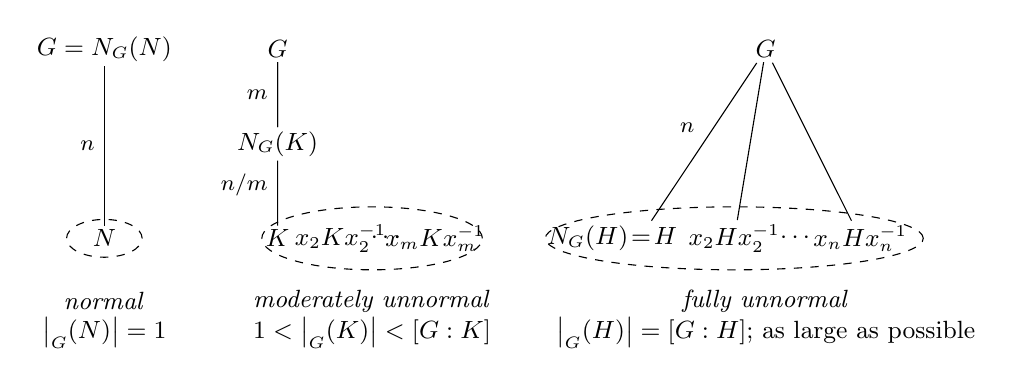
\begin{tikzpicture}[scale=.8]
    \tikzstyle{every node}=[font=\small]
    %%
    \begin{scope}[shift={(0,0)},shorten >= -2pt, shorten <= -2pt]
      \node (G) at (0,3) {$G=\Balert{N_G(N)}$};
      \node (N) at (0,0) {$N$};
      \draw (G)--(N) node[left,pos=.5] {\footnotesize $n$};
      \draw[dashed] (0,0) circle [x radius=.6cm, y radius=.3cm];
      \node at (0,-1) {\Balert{\emph{normal}}};
      \node at (0,-1.5) {$\big|\cl_G(N)\big|=1$};
    \end{scope}
    %%
    \begin{scope}[shift={(4.25,0)},shorten >= -2pt, shorten <= -2pt]
      \node (G) at (-1.5,3) {$G$};
      \node (N_G) at (-1.5,1.5) {\Palert{$N_G(K)$}};
      \node (K) at (-1.5,0) {$K$};
      \node (K2) at (-.5,0) {$x_2Kx_2^{-1}$};
      \node (K3) at (.25,0) {$\cdots$};
      \node (Kl) at (1,0) {$x_m Kx_m^{-1}$};
      \draw (G) -- (N_G);
      \draw (N_G) -- (K) node[left,pos=.35] {\footnotesize $n/m$};
      \draw (G)--(N_G) node[left,pos=.5] {\footnotesize $m$};
      \draw[dashed] (0,0) circle [x radius=1.75cm, y radius=.5cm];
      \node at (0,-1) {\Palert{\emph{moderately unnormal}}};
      \node at (0,-1.5) {$1<\big|\cl_G(K)\big|<[G:K]$};
    \end{scope}
    %%
    \begin{scope}[shift={(10.5,0)},shorten >= -2pt, shorten <= -2pt]
      \node (G) at (0,3) {$G$};
      \node (H) at (-2,0) {\hspace{-7mm}$\Alert{N_G(H)}\!=\!H$};
      \node (H2) at (-.5,0) {$x_2Hx_2^{-1}$};
      \node (H3) at (.5,0) {$\cdots$};
      \node (Hl) at (1.5,0) {$x_n Hx_n^{-1}$};
      \draw (G)--(H) node[above left,pos=.5] {\footnotesize $n$};
      \draw (G) -- (H2); \draw (G) -- (Hl);
      \draw[dashed] (-.5,0) circle [x radius=3cm, y radius=.5cm];
      \node at (0,-1) {\Alert{\emph{fully unnormal}}};
      \node at (0,-1.5) {$\big|\cl_G(H)\big|=[G:H]$; as large as possible};
    \end{scope}
  \end{tikzpicture}
  \]

\end{frame}

%%====================================================================

\begin{frame}{Groups acting on subgroups by conjugation}

  Here is an example of $G=D_3$ acting on its subgroups by a homomorphism $\tau: D_3 \to \Perm(S) \cong S_6$. \vspace{-2mm}

  %% Action graph of D_3 acting on its subgroups
  \[
  \begin{tikzpicture}[scale=.8]
    \tikzstyle{n} = [inner sep=1pt] 
    \tikzstyle{p} = [draw,bend left=30,-stealth]
    \tikzstyle{r-thin} = [draw, eRed, bend left=30, -stealth]
    \tikzstyle{b-thin} = [draw, eBlue, bend left=40, -stealth]
    \tikzstyle{every node}=[font=\small]
    %%
    \begin{scope}[shift={(0,5)}]
      \node [n] (0) at (0,0) {$\tau(1)\quad=\quad$};
      \node [n] (e) at (1,0) {$\<1\>$};
      \node [n] (r) at (2,0) {$\<r\>$};
      \node [n] (f) at (3,0) {$\<f\>$};
      \node [n] (rf) at (4,0) {$\<rf\>$};
      \node [n] (r2f) at (5,0) {$\<r^2f\>$};
      \node [n] (D3) at (6,0) {$D_3$};
    \end{scope}
    %%
    \begin{scope}[shift={(0,4)}]
      \node [n] (0) at (0,0) {\color{xRed} $\tau(r)\quad=\quad$};
      \node [n] (e) at (1,0) {\color{xRed} $\<1\>$};
      \node [n] (r) at (2,0) {\color{xRed} $\<r\>$};
      \node [n] (f) at (3,0) {\color{xRed} $\<f\>$};
      \node [n] (rf) at (4,0) {\color{xRed} $\<rf\>$};
      \node [n] (r2f) at (5,0) {\color{xRed} $\<r^2f\>$};
      \node [n] (D3) at (6,0) {$D_3$};
      \path [r-thin] (f) to (rf);
      \path [r-thin] (rf) to (r2f);
      \path [r-thin] (r2f) to (f);
    \end{scope}
    %%
    \begin{scope}[shift={(0,3)}]
      \node [n] (0) at (0,0) {$\tau(r^2)\quad=\quad$};
      \node [n] (e) at (1,0) {$\<1\>$};
      \node [n] (r) at (2,0) {$\<r\>$};
      \node [n] (f) at (3,0) {$\<f\>$};
      \node [n] (rf) at (4,0) {$\<rf\>$};
      \node [n] (r2f) at (5,0) {$\<r^2f\>$};
      \node [n] (D3) at (6,0) {$D_3$};
      \path [p] (rf) to (f);
      \path [p] (r2f) to (rf);
      \path [p] (f) to (r2f);
    \end{scope}
    %%
    \begin{scope}[shift={(0,2)}]
      \node [n] (0) at (0,0) {\color{xBlue} $\tau(f)\quad=\quad$};
      \node [n] (e) at (1,0) {\color{xBlue} $\<1\>$};
      \node [n] (r) at (2,0) {\color{xBlue} $\<r\>$};
      \node [n] (f) at (3,0) {\color{xBlue} $\<f\>$};
      \node [n] (rf) at (4,0) {\color{xBlue} $\<rf\>$};
      \node [n] (r2f) at (5,0) {\color{xBlue} $\<r^2f\>$};
      \node [n] (D3) at (6,0) {$D_3$};
      \path [b-thin] (rf) to (r2f);
      \path [b-thin] (r2f) to (rf);
    \end{scope}
    %%
    \begin{scope}[shift={(0,1)}]
      \node [n] (0) at (0,0) {$\tau(rf)\quad=\quad$};
      \node [n] (e) at (1,0) {$\<1\>$};
      \node [n] (r) at (2,0) {$\<r\>$};
      \node [n] (f) at (3,0) {$\<f\>$};
      \node [n] (rf) at (4,0) {$\<rf\>$};
      \node [n] (r2f) at (5,0) {$\<r^2f\>$};
      \node [n] (D3) at (6,0) {$D_3$};
      \path [p] (f) to (r2f);
      \path [p] (r2f) to (f);  
    \end{scope}
    %%
    \begin{scope}[shift={(0,0)}]
      \node [n] (0) at (0,0) {$\tau(r^2f)\quad=\quad$};
      \node [n] (e) at (1,0) {$\<1\>$};
      \node [n] (r) at (2,0) {$\<r\>$};
      \node [n] (f) at (3,0) {$\<f\>$};
      \node [n] (rf) at (4,0) {$\<rf\>$};
      \node [n] (r2f) at (5,0) {$\<r^2f\>$};
      \node [n] (D3) at (6,0) {$D_3$};
      \path [p] (f) to (rf);
      \path [p] (rf) to (f);
    \end{scope}
    %%
    \begin{scope}[shift={(9.5,-1.75)},shorten >= -3pt, shorten <= -3pt,
        yscale=1.1]
      \tikzstyle{every node}=[font=\small]
      %%
      \node(G) at (0,6) {$D_3$};
      \node(r) at (-1.75,4.5) {$\<r\>$};
      \node(1) at (0,1.5) {$\<1\>$};
      \node(f) at (.25,24/7) {$\<f\>$};
      \node(rf) at (1.75,24/7) {$\<rf\>$};
      \node(r2f) at (3.25,24/7) {$\<r^2\!f\>$};
      \draw[faded] (G)--(r); 
      \draw[faded] (G)--(f); 
      \draw[faded] (G)--(rf); 
      \draw[faded] (G)--(r2f); 
      \draw[faded] (r)--(1); 
      \draw[faded] (f)--(1);  
      \draw[faded] (rf)--(1); 
      \draw[faded] (r2f)--(1); 
      \draw [r] (f) to (rf);
      \draw [r] (rf) to (r2f);
      \draw [r] (r2f) to [bend left] (f);
      \draw [bb] (rf) to [bend left] (r2f);
      \path (G) edge [r,loop left,>=stealth] (G);
      \path (G) edge [b,loop right,>=stealth] (G);
      \path (r) edge [r,loop left,>=stealth] (r);
      \path (r) edge [b,loop right,>=stealth] (r);
      \path (1) edge [r,loop left,>=stealth] (1);
      \path (1) edge [b,loop right,>=stealth] (1);
      \path (f) edge [b,loop above,>=stealth] (f);
    \end{scope}
  \end{tikzpicture}
  \]
  
  \vspace{-2mm}
  
  \begin{exampleblock}{Observations}
    Do you see how to read stabilizers and fixed points off of the
    permutation diagram? \Pause
    \begin{itemize}
    \item \Balert{$\Ker(\phi)=\<1\>$} consists of the \Balert{row(s)}
      with only fixed points. \Pause
    \item \Galert{$\Fix(\phi)=\big\{\<1\>,\<r\>,D_3\big\}$} consists of the
      \Galert{column(s)} with only fixed points. \Pause
    \item By the orbit-counting theorem, there are
      $|\Alert{\Orb(\phi)}|=24/|D_3|=4$ conjugacy classes.
    \end{itemize}
  \end{exampleblock}
  
\end{frame}

%%====================================================================

\begin{frame}{Groups acting on subgroups by conjugation}

  Here is an example of
  $G=A_4=\<{\color{xRed}(123)},{\color{xBlue}(12)(34)}\>$ acting on its
  subgroups.

  %% Action graph of A_4 acting on its subgroups by conjugation
  \[
  \begin{tikzpicture}[shorten >= -3pt, shorten <= -3pt,auto]
    \tikzstyle{every node}=[font=\normalsize]
    %%
    \begin{scope}[shift={(0,0)},scale=.9]
      \node(A4) at (0,6) {$A_4$};
      \node(V4) at (2.25,4) {$\big\<(12)(34),(13)(24)\big\>$};
      \node(C34) at (-.75,3) {$\big\<(234)\big\>$};
      \node(C33) at (-2.25,3){$\big\<(134)\big\>$};
      \node(C32) at (-3.75,3){$\big\<(124)\big\>$};
      \node(C31) at (-5.25,3) {$\big\<(123)\big\>$};
      \node(C21) at (.75,2) {$\big\<(12)(34))\big\>$};
      \node(C22) at (2.75,2) {$\big\<(13)(24)\big\>$};
      \node(C23) at (4.75,2) {$\big\<(14)(23))\big\>$};
      \node(1) at (0,0) {$\<e\>$};
      \draw[faded] (A4)--(V4);
      \draw[faded] (A4)--(C31);
      \draw[faded] (A4)--(C32);
      \draw[faded] (A4)--(C33);
      \draw[faded] (A4)--(C34);
      \draw[faded] (C31)--(1);
      \draw[faded] (C32)--(1);
      \draw[faded] (C33)--(1);
      \draw[faded] (C34)--(1);
      \draw[faded] (V4)--(C21);
      \draw[faded] (V4)--(C22);
      \draw[faded] (V4)--(C23);
      \draw[faded] (C21)--(1);
      \draw[faded] (C22)--(1);
      \draw[faded] (C23)--(1);
      \path (A4) edge [r,loop left,>=stealth] (A4);
      \path (A4) edge [b,loop right,>=stealth] (A4);
      \path (V4) edge [r,loop above,>=stealth] (V4);
      \path (V4) edge [b,loop below,>=stealth] (V4);
      \path (C31) edge [r,loop above,>=stealth] (C31); 
      \draw [r] (C33) to[bend right=40] (C32);
      \draw [r] (C34) to[bend right=40] (C33);
      \draw [r] (C32) to[bend right=30] (C34);      
      \draw [bb] (C31) to (C32);
      \draw [bb] (C33) to (C34);
      \path (C21) edge [b,loop above,>=stealth] (C21);
      \path (C22) edge [b,loop above,>=stealth] (C22);
      \path (C23) edge [b,loop above,>=stealth] (C23);
      \path (1) edge [r,loop left,>=stealth] (1);
      \path (1) edge [b,loop right,>=stealth] (1);
      \draw [r] (C22) to[bend right=35] (C21);
      \draw [r] (C23) to[bend right=35] (C22);
      \draw [r] (C21) to[bend right=25] (C23);
    \end{scope}
  \end{tikzpicture}
  \]
  
  Let's take a moment to revisit our ``\emph{three favorite examples}''
  from Chapter 3.
  \[
  N=\big\<(12)(34),(13)(24)\big\>,\qquad H=\big\<(123)\big\>,\qquad K
  =\big\<(12)(34)\big\>.
  \]
  
\end{frame}

%%====================================================================

\begin{frame}{Groups acting on subgroups by conjugation}
  
  Here is the ``\emph{fixed point table}'' of the action of $A_4$ on
  its subgroups.
  \[
  \hspace{-5mm}
  \scalebox{.77}{
    \begin{tikzpicture}
      \node at (0,0) {
        \renewcommand\arraystretch{1.7}
        \begin{tabular}{c|cccccccccc}
          & {\small$\<e\>$} & {\small$\<(123)\>$} & {\small$\<(124)\>$} & {\small$\<(134)\>$} & {\small$\<(234)\>$} & {\small$\<(12)(34)\>$} & {\small$\<(13)(24)\>$} & {\small$\<(14)(23)\>$} & {\small$\<(12)(34),(13)(24)\>$} & {\small $A_4$} \\ \hline
          \small $e$ & \checkmark & \checkmark & \checkmark & \checkmark & \checkmark & \checkmark & \checkmark & \checkmark & \checkmark & \checkmark \\
\small $(123)$ & \checkmark & \checkmark & & & & & & & \checkmark & \checkmark \\
\small $(132)$ & \checkmark & \checkmark & & & & & & & \checkmark & \checkmark \\
\small $(124)$ & \checkmark & & \checkmark & & & & & & \checkmark & \checkmark \\
\small $(142)$ & \checkmark & & \checkmark & & & & & & \checkmark & \checkmark \\
\small $(134)$ & \checkmark & & & \checkmark & & & & & \checkmark & \checkmark \\
\small $(143)$ & \checkmark & & & \checkmark & & & & & \checkmark & \checkmark \\
\small $(234)$ & \checkmark & & & & \checkmark & & & & \checkmark & \checkmark \\
\small $(243)$ & \checkmark & & & & \checkmark & & & & \checkmark & \checkmark \\
\small $(12)(34)$ & \checkmark & & & & & \checkmark & \checkmark & \checkmark & \checkmark & \checkmark \\
\small $(13)(24)$ & \checkmark & & & & & \checkmark & \checkmark & \checkmark & \checkmark & \checkmark \\
\small $(14)(23)$ & \checkmark & & & & & \checkmark & \checkmark & \checkmark & \checkmark & \checkmark \\
      \end{tabular}};
  \end{tikzpicture}}
  \]
  
  \Pause
  
  By the \textbf{orbit-counting theorem}, there are 
  $|\Orb(\phi)|=60/|A_4|=5$ conjugacy classes. 
  
\end{frame}

%%====================================================================

\begin{frame}{A summary}
  
  Thus far, we have seen four important (right) actions of a group $G$, acting:

  \begin{itemize}
  \item on itself by multiplication
  \item on itself by conjugation. 
  \item on its subgroups by conjugation. 
  \item on the cosets of a fixed subgroup $H\leq G$ by
    multiplication.
  \end{itemize}
  
  \bigskip  
  \scalebox{.95}{  
    \def\arraystretch{1.75}
    \begin{tabular}{|c|cccc|} \hline
      set $S=$ & \multicolumn{2}{c}{$G$} & subgroups of $G$ & right cosets of $H$ \\ \hline
      operation & multiplication & conjugation  & conjugation &  right multiplication \\ \hline
      $\orb(s)$ & $G$ & $\cl_G(g)$ & $\cl_G(H)$ & all right cosets \\
      $\stab(s)$ & $\<1\>$ & $C_G(g)$ & $N_G(H)$ & $x^{-1}Hx$ \\
      $\fix(g)$ & $G$ or $\emptyset$ & $C_G(g)$ & $\{H\mid g\in N_G(H)\}$ & $\big\{Hx\mid xgx^{-1}\in H\big\}$ \\
      $\Ker(\phi)$ & $\<1\>$ & $Z(G)$ & $\displaystyle\bigcap_{H\leq G} N_G(H)$ &
      largest norm. subgp. $N\leq H$ \\
      $\Fix(\phi)$ & $\emptyset$ & $Z(G)$ & normal subgroups & none \\ \hline
  \end{tabular}}
  
\end{frame}

%%====================================================================

\section{More applications of group actions!}

\begin{frame}{Here is where we did a fun example in class}
  In class we talked about $SA_8$ acting on itself by conjugation:
  \begin{itemize}
    \item we drew an action diagram, \medskip
    \item we drew boxes around each orbit, \medskip
    \item we looked at fixators, \medskip
    \item we looked at fixed points, which was $Z(SA_8) = \<r^2\>$, \medskip
    \item and we said that $|SA_8| = (4\cdot 1) + 2 + 2 + 2 + 2 + 2 + 2$.
  \end{itemize}
\end{frame}

%%====================================================================
\section*{Cauchy's theorem}
\begin{frame}{A creative application of a group action}

  \begin{block}{Cauchy's theorem} 
    If $p$ is a prime dividing $|G|$, then $G$ has an element (and
    hence a subgroup) of order $p$.
  \end{block}
  
  \begin{exampleblock}{Proof} \Pause
    Let $P$ be the set of ordered $p$-tuples of
    elements from $G$ whose product is $e$: \vspace{-1mm}
    \[
    (x_1,x_2,\dots,x_p)\in P\quad\mbox{iff}\quad x_1x_2\cdots
    x_p=e\,. \Pause
    \]
    Observe that $|P|=|G|^{p-1}$. (We can choose
    $x_1,\dots,x_{p-1}$ freely; then $x_p$ is forced.)
    
    \pause\medskip 
    
    The group $\Z_p$ acts on $P$ by cyclic shift: \vspace{-2
      mm}
    \[
    \phi\colon\Z_p\longrightarrow\Perm(P),\qquad
    (x_1,x_2,\dots,x_p)\stackrel{\phi(1)}{\longmapsto}
    (x_2,x_3\dots,x_p,x_1)\,. %\Pause
    \]
    \Pause The set $P$ is partitioned into orbits, each of size
    $|\orb(s)|=[\Z_p:\stab(s)]=1$ or $p$.
        
    \pause\medskip
    
    The only way that the orbit of $(x_1,x_2,\dots,x_p)$
    can have size $1$ is if $x_1=\cdots=x_p$.

    \Pause\medskip

    Clearly, $(e,\dots,e)\in P$ is a fixed point.
    
    \Pause\medskip
    
    The $|G|^{p-1}-1$ other elements in $P$ sit in orbits of size $1$
    or $p$.
    
    \pause\medskip
    
    Since $p\nmid |G|^{p-1}-1$, there must be other orbits of size
    $1$. \Pause Thus, some $(x,\dots,x)\in P$, with $x\neq e$ satisfies
    $x^p=e$. $\hfill\Box$
  \end{exampleblock}
  
\end{frame}

%%====================================================================

\begin{frame}{Classification of groups of order 6} %\Pause

  By Cauchy's theorem, every group of order $6$ must have:
  \begin{itemize}
  \item an element $\Alert{a}$ of order $3$
    \item an element $\Balert{b}$ of order $2$.
  \end{itemize}
      
  \medskip\Pause

  Clearly, $G=\<\Alert{a},\Balert{b}\>$, and so
   $G$ must have the following ``partial  Cayley graph'':
  %%
  %% Partial Cayley graph of a group of order 6
  \[
  \begin{tikzpicture}[scale=1.1,auto]
    \tikzstyle{every node}=[font=\footnotesize]
    %%
    \node (b) at (0,0) [v] {$b$};
    \node (e) at (0,1) [v] {$e$};
    \node (ba) at (1,0) [v] {$ba$};
    \node (a) at (1,1) [v] {$a$};
    \node (ba2) at (2,0) [v] {$ba^2$};
    \node (a2) at (2,1) [v] {$a^2$};
    \draw [r] (e) to (a); \draw [r] (a) to (a2);
    \draw [r] (a2) to [bend right] (e);
    \draw [r] (b) to (ba); \draw [r] (ba) to (ba2);
    \draw [r] (ba2) to [bend left] (b);
    \draw [bb] (e) to (b);
  \end{tikzpicture}
  \]
  \Pause It is now easy to see that up to isomorphism, there are only $2$
  groups of order $6$: \Pause
  \[
  \begin{tikzpicture}[scale=1.1,auto]
    \tikzstyle{every node}=[font=\footnotesize]
    %%
    \node at (-1.5,.5) {\normalsize $C_6\cong C_2\times C_3$};
    \node (b) at (0,0) [v] {$b$};
    \node (e) at (0,1) [v] {$e$};
    \node (ba) at (1,0) [v] {$ba$};
    \node (a) at (1,1) [v] {$a$};
    \node (ba2) at (2,0) [v] {$ba^2$};
    \node (a2) at (2,1) [v] {$a^2$};
    \draw [r] (e) to (a); \draw [r] (a) to (a2);
    \draw [r] (a2) to [bend right] (e);
    \draw [r] (b) to (ba); \draw [r] (ba) to (ba2);
    \draw [r] (ba2) to [bend left] (b);
    \draw [bb] (e) to (b);
    \draw [bb] (a) to (ba);
    \draw [bb] (a2) to (ba2);      
  \end{tikzpicture}
  \qquad\qquad\qquad\Pause
  \begin{tikzpicture}[scale=1.1,auto]
    \tikzstyle{every node}=[font=\footnotesize]
    \node at (2.75,.5) {\normalsize $D_3$};
    \node (b) at (0,0) [v] {$b$};
    \node (e) at (0,1) [v] {$e$};
    \node (ba) at (1,0) [v] {$ba$};
    \node (a) at (1,1) [v] {$a$};
    \node (ba2) at (2,0) [v] {$ba^2$};
    \node (a2) at (2,1) [v] {$a^2$};
    \draw [r] (e) to (a); \draw [r] (a) to (a2);
    \draw [r] (a2) to [bend right] (e);
    \draw [r] (b) to (ba); \draw [r] (ba) to (ba2);
    \draw [r] (ba2) to [bend left] (b);
    \draw [bb] (e) to (b);
    \draw [bb] (a) to (ba2);
    \draw [bb] (a2) to (ba);      
  \end{tikzpicture}
  \]
  \Pause \textbf{Exercise}. Suppose that $|G| = pq$, where $p < q$ are primes and $p$ doesn't divide $q-1$. Prove that $G$ is cyclic.
  
\end{frame}

%%====================================================================

\section*{The end!}
%%====================================================================

\end{document}
